\documentclass[tikz,border=10pt]{standalone}
\usetikzlibrary{mindmap}
\begin{document}
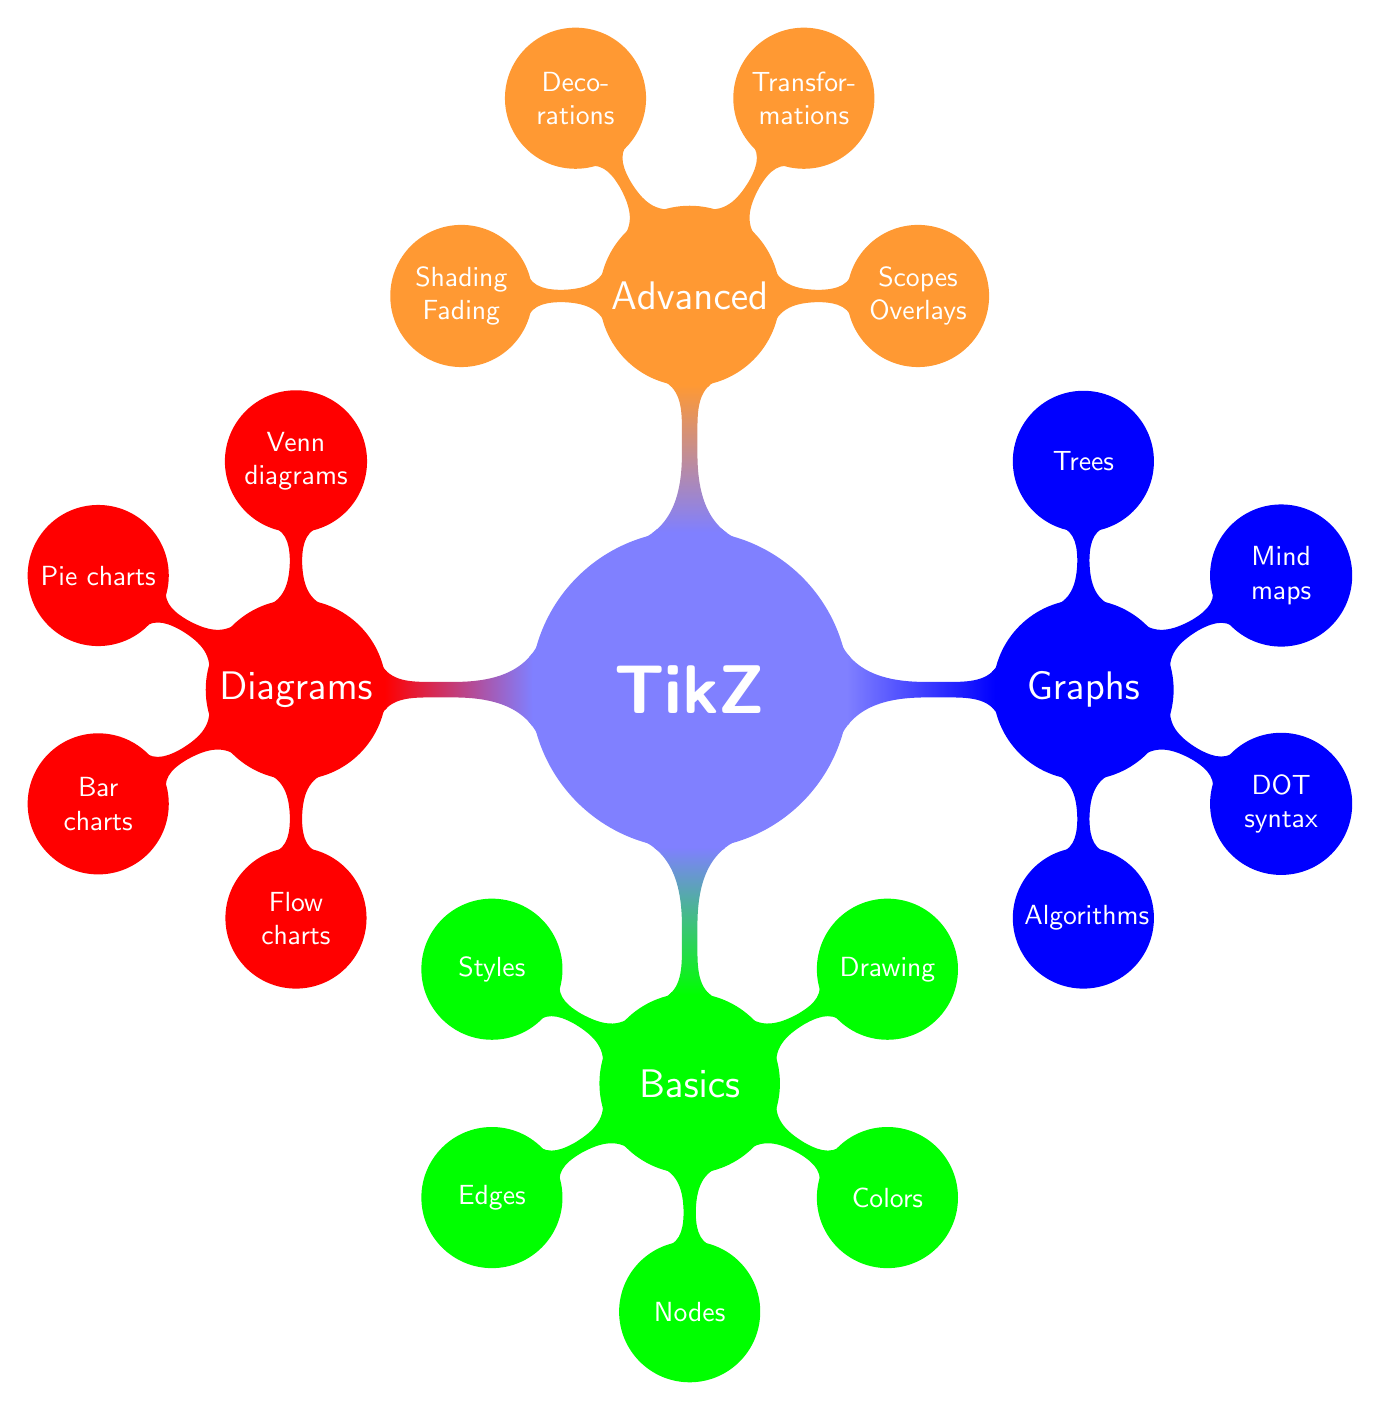
\begin{tikzpicture}[
  mindmap,
  text = white,
  concept color = blue!50,
  nodes = {concept},
  root/.append style = {
    font = \Huge\sffamily\bfseries},
  level 1 concept/.append style =
    {font = \Large\sffamily, sibling angle=90},
  level 2 concept/.append style =
    {font = \normalsize\sffamily}
  ]
  \node [root] {TikZ} [clockwise from=0]
    child [concept color=blue] {
      node {Graphs} [clockwise from=90]
        child { node {Trees} }
        child { node {Mind maps} }
        child { node {DOT syntax} }
        child { node {Algorithms} }
    }
    child [concept color=green] {
      node {Basics} [clockwise from=30]
        child { node {Drawing} }
        child { node {Colors} }
        child { node {Nodes} }
        child { node {Edges} }
        child { node {Styles} }
    }
    child [concept color=red] {
      node {Diagrams} [clockwise from=-90]
        child { node {Flow charts} }
        child { node {Bar charts} }
        child { node {Pie charts} }
        child { node {Venn diagrams} }
    }
    child [concept color=orange!80] {
      node {Advanced} [clockwise from=180]
        child { node {Shading\\Fading} }
        child { node {Deco\-rations} }
        child { node {Transfor\-mations} }
        child { node {Scopes\\Overlays} }
    };
\end{tikzpicture}
\end{document}
